\documentclass{article}
\usepackage{amssymb, amsmath, amsthm}
\usepackage[margin=1in]{geometry}
\usepackage{verbatim}
\usepackage{graphicx}
\usepackage{hyperref} % \url \href
\usepackage{docmute}

\newtheorem{definition}{Definition}
\newtheorem{theorem}{Theorem}
\DeclareMathOperator{\spn}{Span}

\usepackage[style=chem-acs ,backend=bibtex, sorting=none]{biblatex}
\addbibresource{autoTB.bib}

\begin{document}


\section{Tight-binding Method}
\subsection{Tight-binding approximation}
Tight-binding methods is a well known technique to solve the band structure of 
crystalline material with a model Hamiltonian\cite{ziman_principles_1999}. 
It is fast to run and is able to 
reproduce the DFT calculated band structure accurately provided a suitable set of 
parameters. 
In the tight binding approximation, we write the Hamiltonian in the local 
basis orbitals:
\begin{equation}
    H_{ij}(R) = \langle \phi_{R',i} | H | \phi_{R'+R,j} \rangle = \langle \phi_{0,i} | H | \phi_{R,j} \rangle
\end{equation}
where index 0, $R$ refer to an arbitrarily selected `home' unitcell and unit cell at 
lattice vector $R$. The Bloch-like basis functions are then:
\begin{equation}
    |\psi_j^k\rangle = \sum_R e^{ik\cdot(R+t_j)} |\phi_{Rj} \rangle
\end{equation}
and the Hamiltonian matrix at reciprocal vector $\mathbf{k}$ is related to the 
Hamiltonian in real space by:
\begin{equation}
    H_{ij}^{\mathbf{k}} = \langle \psi_i^k | H |\psi_j^k\rangle = \sum_R e^{ik\cdot(R+t_j-t_i)} = H_{ij}(R)
\end{equation}
Diagonalizing the square matrix $H_{ij}^{\mathbf{k}}$ gives the eigen energies at $\mathbf{k}$
in the tight-binding approximation. 

\subsection{Solving the density of states}
Given a tight-binding model, the electronic density of states can be found by solving the 
Hamiltonian on a regularly spaced $\mathbf{k}$-grid, and straightforwardly calculated 
by numerical intergration methods, such as a summation of Gaussian peaks or tetrahedron methods. 

\section{Method}
\subsection{Work flow}
Our work concern the learning of a tight-binding approximation of crystalline materials 
with atomic orbitals as basis functions. The key approximation in this work is the 
nearest neighbor interaction approximation for the tight-binding interaction matrix elements. 
Furthermore, symmetry relationship is used to reduce the number of tight-binding parameters.
After obtaining the tight-binding model, the approximate band structure can be calculated 
by diagonalizing the Hamiltonian at the given $\mathbf{k}$ point. 

The overall workflow of our work is as follows in Figure \ref{F:forward_workflow}.
\begin{figure}[h]
    \centering
    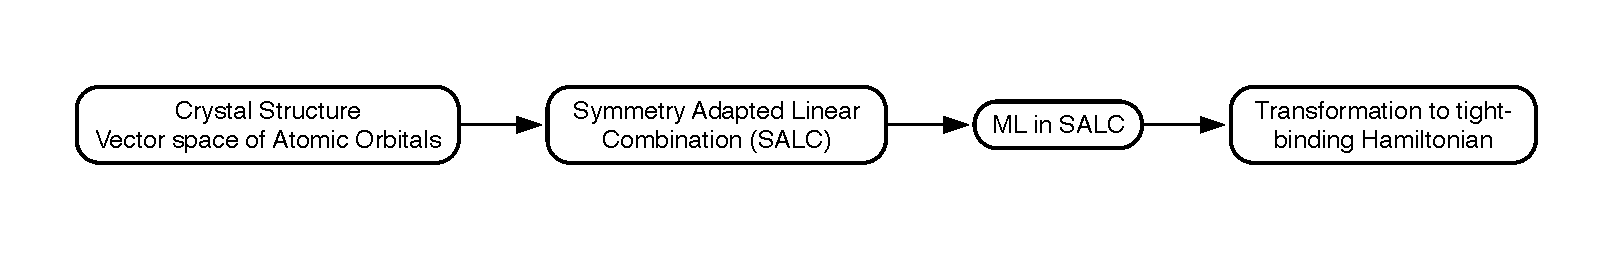
\includegraphics[width=5in]{../figures/forward_workflow.pdf}
    \caption{Prediciton work flow of the tight-binding model generation process}
    \label{F:forward_workflow}
\end{figure}
For an atom $i$ in the input structure and a given set of atomic orbitals on $i$ and its neighbors as basis functions, 
we first identify site symmetry of this cluster and find the symmetry adapted linear combination as molecular orbitals (MO) basis 
functions corresponding to different representations. If two MOs belong to different irreducible representation, we simply 
set their interaction to be zero, otherwise, we use ML to predict their matrix elements. 
From the interactions in MO basis functions, we can apply transformation from MO to AO again, which yield the tight-binding 
Hamiltonian in atomic orbital basis functions.
Detailed treatment are presented in the following sections. 

\subsection{Symmetry adapted linear combinations}
According to the result from application of group theory in quantum chemistry, it can be 
shown that the eigenfunction of the Hamiltonian occupy differrent subgroups, each 
corresponding to a representation of the group of symmetry operation. Given a set of 
functions, the vector space span by them can be written as a direct sum of these 
\emph{invariant subspace}, and we can project any arbitrary functions into different 
components corresponding to these representations. This procedure is based on characters 
of the group representations and the orthogonal theorem for characters\cite{dresselhaus_group_2008}. 
For a detailed treatment and introduction to the method, see Appendix A.

Let's consider the example of group $D_{3h}$ corresponding to a molecular with one atom sitting 
on the origin and three atoms sitting on each tip of triangle lying in the $xy$ plane. We consider 
the three dimensional vector space span by three $s$ functions on each of the three atoms:
\begin{equation}
    V = \spn(|s_1\rangle, |s_2\rangle, |s_3\rangle)
\end{equation}
The projection operator into each invariant subspace of the representation $\Gamma_i$ is given by:
\begin{equation}
    P^{\Gamma_i} = \frac{l_i}{h} \sum_R \chi^{\Gamma_i}(R) P_R
\end{equation}
where $l_i$ is the dimension of the representation, $h$ is the order of the group, 
$\chi^{\Gamma_i}(R)$ is the character of the symmetry operation $R$ in this representation 
and $P_R$ is the symmetry operator in the basis of $|s_1\rangle, |s_2\rangle, |s_3\rangle$. 
Applying the projection operator onto each basis function, for all the representation, 
gives the result:
\begin{equation}
    | \psi^{A_1'} \rangle = P^{A_1'}|s_1\rangle = P^{A_1'}|s_2\rangle = P^{A_1'}|s_3\rangle 
    = \frac{\sqrt{3}}{3} (|s_1\rangle + |s_2\rangle + |s_3\rangle)
\end{equation}
which give the basis vector for the one dimensional subspace of representation $A_1'$, 
we also have:
\begin{align}
    |\psi_1^{E'}\rangle &= P^{E'} | s_1 \rangle = \frac{\sqrt{6}}{6}(\ \ \ 2|s_1\rangle - |s_2\rangle - |s_3\rangle) \\
    |\psi_2^{E'}\rangle &= P^{E'} | s_2 \rangle = \frac{\sqrt{6}}{6}(- |s_1\rangle + 2|s_2\rangle - |s_3\rangle) \\
    |\psi_3^{E'}\rangle &= P^{E'} | s_3 \rangle = \frac{\sqrt{6}}{6}(- |s_1\rangle - |s_2\rangle + 2 |s_3\rangle) \\
\end{align}
for the two dimension representation $E'$, where we find $|\psi_3^{E'}\rangle = - (|\psi_1^{E'}\rangle + |\psi_2^{E'}\rangle)$
showing that the three function projected indeed form a two dimensional subspace. 

After separating the invariant subspaces into different irreducible representations, the problem remains to 
find the suitable basis functions. 
To do so, we use the fact that a irreducible representation become 
reducible when the number of symmetric decreases. 
The functions belong to the irreducible representation of the symmetry group will split into different 
irreducible representation of the subgroup, each exhibit symmetry properties with respect to the reminding 
symmetry operations. 

As an example, in $D_{3h}$, any function in the subspace $E'$ can be written as a linear combination
of two of the three projected functions $|\psi_1^{E'}\rangle$, $|\psi_2^{E'}\rangle$ and $|\psi_3^{E'}\rangle$. 
By descending down symmetry to group $C_s$, which is a subgroup 
of $D_{3h}$ with only two elements: $\{E, \sigma_v\}$ where $\sigma_v$ is one of the three vertical reflection, 
choosen arbitrarily, $E'$ splits into two one dimensional representation $A'_{C_s}$ and $A''_{C_s}$.
Projection of the three functions in $E'$ with character table of $C_s$ yield 
one basis function for each one-dimensional representation:
\begin{align}
    |\psi^{E'\to A'} \rangle &= \frac{2}{\sqrt{6}} |s,2\rangle - \frac{1}{\sqrt{6}} |s,1\rangle - \frac{1}{\sqrt{6}} |s,3\rangle \\
    |\psi^{E'\to A''}\rangle &= \frac{\sqrt{2}}{2} |s,1\rangle - \frac{\sqrt{2}}{2} |s,3\rangle
\end{align}
Being the one dimensional representation of $C_s$, we can identify them to be 
symmetric and anti-symmetric under vertical mirror reflection. 

\subsection{Symmetry Adapted Tight-binding methods}
To simplify the machine learning problem, we focus on reducing the number of parameters 
in the tight-binding model that machine learning method need to predict. First, we utilize 
the fact that the interaction between atomic orbitals basis functions decay fast 
in real space. In the simplest case, only nearest neighbor interaction can be considered. 
Suppose that the average number of neighbors is $N_n$ and we have $N_{ao}$ basis functions 
on each atom, we would have:
\begin{equation}
    \text{Number of interaction} = ( N_n + 1 ) N_{ao}^2 / 2
\end{equation}
where division by $2$ remove the double counting (assuming the Hamiltonian is real, and 
therefore $\langle \phi_1 | H | \phi_2 \rangle = \langle \phi_2 | H | \phi_1 \rangle$). 

On the other hand, a tight-binding model with the nearest neighbor interaction can be further 
simplified using the result from symmetry analysis, and it turns out that 
symmetry restrict the value of and relationship between the matrix elements. 
The key point here is to consider the interaction in terms of MOs.
To illustrate the idea, we use the above example of a molecular in $D_{3h}$ symmetry and 
study the tight-binding parameter between the $|s\rangle$ on $|p_x\rangle$, $|p_y\rangle$
and $|p_z\rangle$ orbital on the origin. 
The three $p$ oribtal can be classified to be of representation 
$|p_z\rangle: A'$, 
$|p_x\rangle: E'\to A'$ and 
$|p_y\rangle: A'\to A''$. 

Since bonding can only be non-zero between vectors in the same representation, for $p_z$ we have
the following linear equation
\begin{align*}
    \frac{\sqrt{3}}{3} (\langle p_z | H | s_1 \rangle + \langle p_z | H | s_2 \rangle + \langle p_z | H | s_3 \rangle) = A \\
    \frac{\sqrt{6}}{6} (2\langle p_z | H | s_2 \rangle - \langle p_z | H | s_1 \rangle - \langle p_z | H | s_3 \rangle) = 0 \\
    \frac{\sqrt{2}}{2} ( \langle p_z | H | s_1 \rangle - \langle p_z | H | s_2 \rangle) = 0
\end{align*}
where $A$ stand for some arbitrary parameter. Solving this linear 
equation give the result:
\begin{equation}
    \langle p_z | H | s_1 \rangle = \langle p_z | H | s_2 \rangle = \langle p_z | H | s_3 \rangle = a
\end{equation}
which agrees with the symmetry relationship between the orbits.
Similarly, for $p_x$ and $p_y$ orbital and let $s_2$ on the $x$ axis. we can find:
\begin{gather}
    2 \langle p_x | H | s_1 \rangle = - \langle p_x | H | s_2 \rangle = 2 \langle p_x | H | s_3 \rangle = b \\
    \langle p_y | H | s_2 \rangle = 0;\quad \langle p_y | H | s_1 \rangle = - \langle p_y | H | s_1 \rangle = c
\end{gather}
so that only three parameter is required to describe nearest neighbor tight binding interaction between the 
$p$ orbitals at the center and the $s_i$ for $i = 1,2,3$:
\begin{table}[h]
    \caption{Interaction matrix elements}
    \label{T:interaction_D_3h}
    \centering
    \begin{tabular}{|c|ccc|}
        \hline
        $\langle \psi_1 | H | \psi_2 \rangle$ & $s_1$ & $s_2$ & $s_3$ \\ \hline
        $p_x$ & $b/2$ & $-b$ & $b/2$ \\
        $p_y$ & $c$ & $0$ & $-c$\\
        $p_z$ & $a$ & $a$ & $a$ \\
        \hline
    \end{tabular}
\end{table}


\subsection{Machine learning Matrix elements}

\newpage

\subsection{Deep Tensor Neural Network (DTNN)}
To utilize the symmetry relationship in the first way, we use the equivariant neural network
structure purposed by Thomas et al.\cite{thomas_tensor_2018} (Deep Tensor Neural Network). 
The network structure (DTNN) is reviewed in Appendix B. 
An important point that separate the equivariant network with general networks using 
invariant descriptors is that the transformation properties are kept in all layers of the equivariant
network such as one purposed by Thomas et al, but transformation properties are not kept if we 
use invariant descriptors. For example, the output of DTNN will change sign for a scalar output  
if a $\pi$ rotation is applied to an $p$ orbital, while the output will be the same for any
simple invariant network. This is one of the key property that we desire.
Furthermore, data in DTNN naturally flow in the form of tensor, which allow us to define 
tensor product, as in the case of Hamiltonian.

\subsection{Using the equivariant network}
Our network take inputs as two vectors and produce a scalar number. Since DTNN's output is 
also vector quantity, we define the network as $H(i,j)$ that operate on vector $| \psi_j \rangle$
\begin{equation}
    H |\psi\rangle = H(| \psi_i \rangle,| \psi_j \rangle) | \psi_j \rangle
\end{equation}
so that the tight-binding matrix element is naturally:
\begin{equation}
    H_{ij} = \langle \psi_i | H | \psi_j \rangle
\end{equation}
DTNN is rotational equivariant, meaning that we have: $H R | \psi_j \rangle  = RH | \psi_j \rangle $, 
as in a general equivariant network, 
where $R$ is an symmetry operation. 

let's now we consider how to use the above result to reduce the number of 
tight-binding matrix element to learn. 
We focus on nearest neighbor interaction and consider the above example, where
we place $p_x$ orbital at the center and two $s^1$, $s^2$ orbitals at $r_1 = (1,0,0)$ and $r_2 = (-1,0,0)$. 
How $s^1$ transform to $s^2$ is not unique, but we consider a $C_2$ rotation for concreteness. 
However, we do not include translation in our consideration but only the point group 
operations (vector transformation). 

Knowing the energy $\langle p_x | H | s^1 \rangle$, how do we derive the energy 
of $\langle p_x | H | s^2 \rangle$? Since $| s^2 \rangle = R | s^1 \rangle$ We have:
\begin{equation}
    \langle p_x | H | s^2 \rangle = \langle p_x | H R | s^1 \rangle
    = \langle p_x | R H | s^1 \rangle = \langle R^{-1} p_x | H | s^1 \rangle
\end{equation}
Since we know how rotation transform $p_x$, we recover the relationship 
\begin{equation}
    \langle p_x | H | s^2 \rangle = - \langle p_x | H | s^1 \rangle
\end{equation}

As a second example, let's consider $pp_{\sigma}$ bond, replacing $s^1$ with $p_x^1$ 
and $s^2$ with $-p_x^2$. Note the negative sign ensures that two orbitals at $r_1$ and $r_2$
are generated by point group symmetry. 
We have:
\begin{equation}
    - \langle p_x^0 | H | p_x^2 \rangle =  - \langle p_x^0 | HR | p_x^1 \rangle 
    = - \langle p_x^0 | RH | p_x^1 \rangle = \langle p_x^0 | H | p_x^1 \rangle
\end{equation} 
which is again the correct results. 


\end{document}
